\documentclass{report}
\usepackage[utf8]{inputenc}
\usepackage{amsmath}
\usepackage{amsthm}
\usepackage{amssymb}
\usepackage{geometry}
\usepackage{mathtools}
\usepackage{cancel}
\usepackage{xfrac}
\usepackage{siunitx} % for scientific notation \num{}
\usepackage{authblk} % for authors
\usepackage{tikz} % for circled{}
\usepackage{systeme} % for system of equations bracket
\usepackage{verbatim} % for comment
\usepackage{xfp} % for floating point operations in macros
\usepackage{graphicx} % for cropping the images
\usepackage{dsfont} % for doublestroke fonts
\usepackage{float}
\usepackage[colorlinks=true,citecolor=blue]{hyperref} % hyperlink
\usepackage[scr=rsfso,frak=euler,bb=ams]{mathalfa} % math letters
\usepackage[english]{babel}
\usepackage[square,numbers]{natbib}
\bibliographystyle{abbrvnat}

\begin{document}

\begin{center}
    \Large Quadcopter Dynamics and Numerical Simulation \\
    \large MAE 542 Final Project Proposal \\
    \vspace{0.5em}
    \small Matthew Coleman \\
    \small November 22, 2022
\end{center}

\begin{figure}[H]
    \centering
    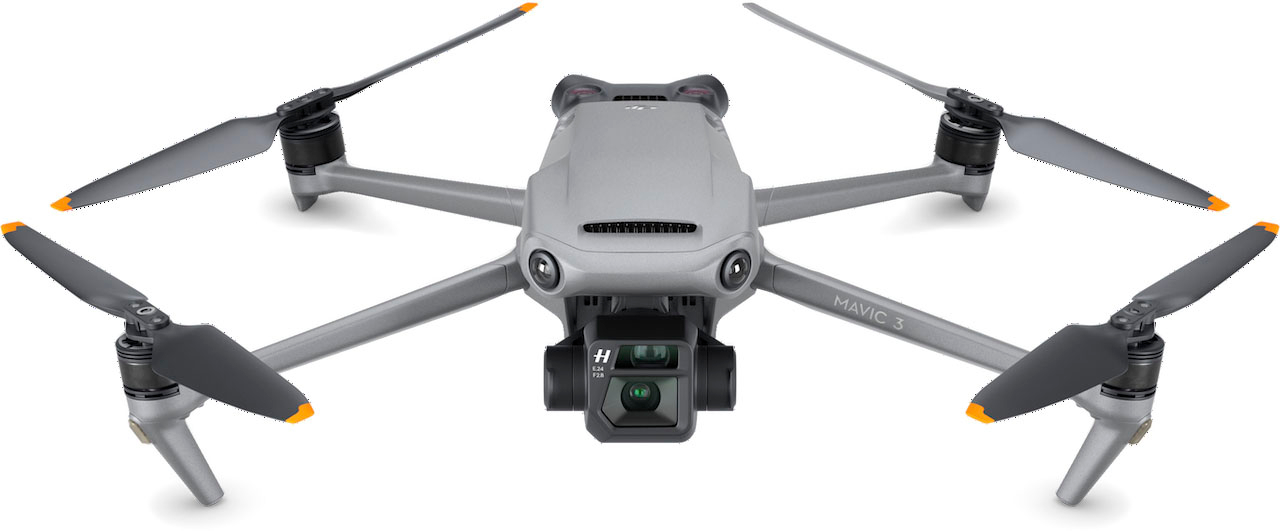
\includegraphics[width=0.7\textwidth]{proposal/quadcopter.jpg}
    \caption{DJI Mavic 3 Quadcopter}
    \label{fig:quadcopter_image}
\end{figure}

\section{Introduction}

A quadcopter is a helicopter with four propellers arranged in a square formation. It can be controlled by rapidly changing the angular velocity of each rotor independently, such that a directional thrust and torque can be achieved about the body of the drone. They have a wide variety of uses including aerial photography, search and rescue, agriculture, and surveillance \cite{luukkonen2011modelling}.

Although the structure is simple to construct and models are widely accessible on consumer markets, the dynamics and control systems required to make any use of the physical system are complex and nonlinear. In addition, quadcopters can be expensive and difficult to learn to control for a human operator. Thus, the setting is ideal for rigorous dynamical analysis, and a comprehensive numerical simulation of the quadrotor dynamics would be particularly helpful for people that wish to learn how to pilot one without running the risk of destroying it accidentally.

\section{Methodology}

I propose a project that adheres to the ``Application Project'' description in two parts, including the derivation and explanation of the quadrotor dynamics using the Lagrangian formulation as well as an implementation of these dynamics in python using numerical integration. While these are the bare minimum I propose for the project, further work could include an implementation of a rudimentary control system or input to the real-time simulation, such that the program could be used as a piloting simulation, following in the methodology of \cite{murphy2016modular}.

\bibliography{main}

\end{document}
